% P05 diagnostic figure source_vs_held|development|M01; allowlisted public aggregate points.
% Each point is an aggregate mean or bin over repeated contexts, not an independent sample.
% data_sha256=7f60e425b5fe235c362c21442c3237e1521aad33df8bebdebfd5854e0cfadd4b
\documentclass[tikz,border=5pt]{standalone}
\ifdefined\pdfinfoomitdate\pdfinfoomitdate=1\fi
\ifdefined\pdfsuppressptexinfo\pdfsuppressptexinfo=-1\fi
\ifdefined\pdftrailerid\pdftrailerid{}\fi
\usepackage{pgfplots}
\usepgfplotslibrary{groupplots}
\pgfplotsset{compat=1.18}
\definecolor{p05Blue}{HTML}{0072B2}
\definecolor{p05Orange}{HTML}{E69F00}
\definecolor{p05Green}{HTML}{009E73}
\definecolor{p05Purple}{HTML}{CC79A7}
\definecolor{p05Red}{HTML}{D55E00}
\definecolor{p05Sky}{HTML}{56B4E9}
\begin{document}
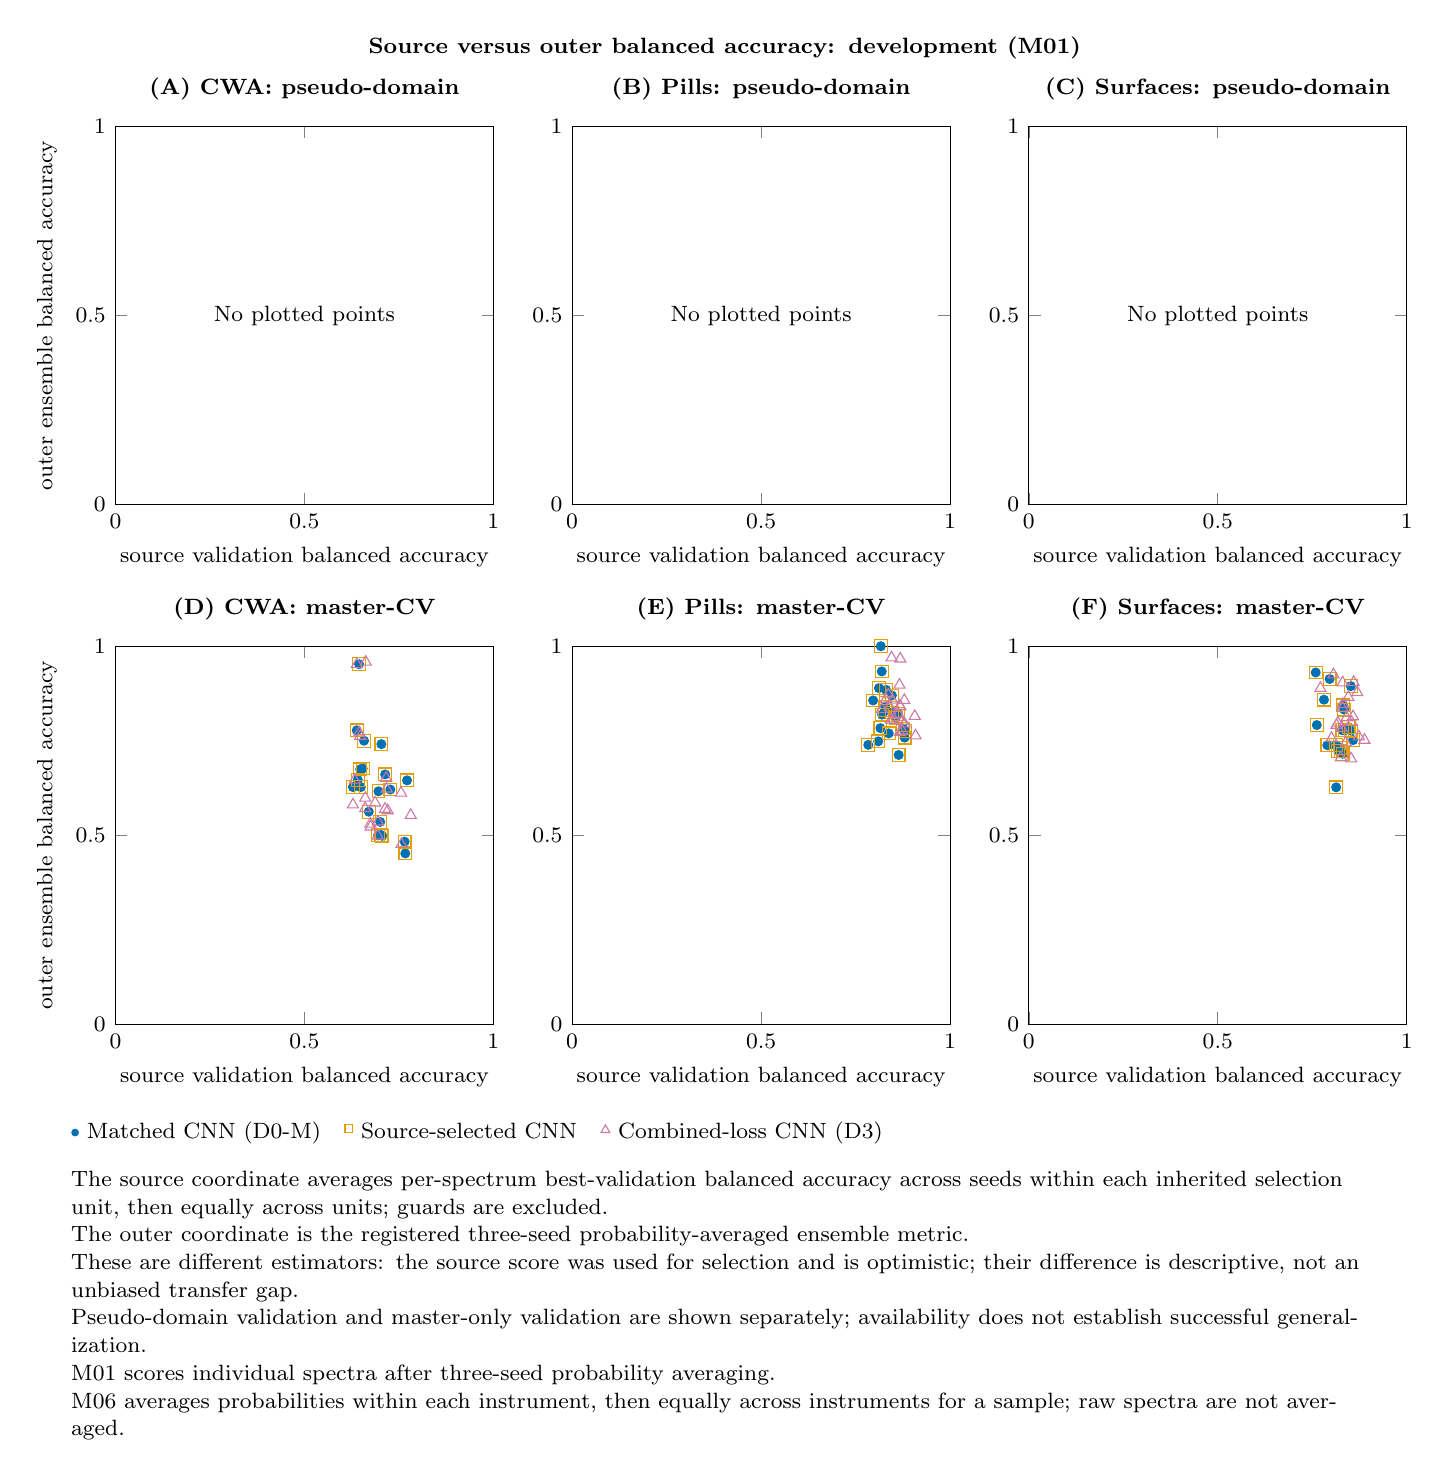
\begin{tikzpicture}
\begin{groupplot}[
  group style={group size=3 by 2, horizontal sep=1.0cm, vertical sep=1.8cm},
  width=4.8cm, height=4.8cm, scale only axis,
  xmin=0, xmax=1, ymin=0, ymax=1,
  xtick={0,0.5,1}, ytick={0,0.5,1},
  tick label style={font=\fontsize{8}{10}\selectfont, color=black},
  label style={font=\fontsize{8}{10}\selectfont, color=black},
  title style={font=\fontsize{8}{10}\selectfont\bfseries, color=black},
]
\nextgroupplot[title={(A) CWA: pseudo-domain}, xlabel={source validation balanced accuracy}, ylabel={outer ensemble balanced accuracy}]
\node[font=\fontsize{8}{10}\selectfont,align=center] at (axis cs:0.5,0.5) {No plotted points};
\nextgroupplot[title={(B) Pills: pseudo-domain}, xlabel={source validation balanced accuracy}]
\node[font=\fontsize{8}{10}\selectfont,align=center] at (axis cs:0.5,0.5) {No plotted points};
\nextgroupplot[title={(C) Surfaces: pseudo-domain}, xlabel={source validation balanced accuracy}]
\node[font=\fontsize{8}{10}\selectfont,align=center] at (axis cs:0.5,0.5) {No plotted points};
\nextgroupplot[title={(D) CWA: master-CV}, xlabel={source validation balanced accuracy}, ylabel={outer ensemble balanced accuracy}]
\addplot[only marks, mark=*, mark size=1.6pt, color=p05Blue, mark options={fill=p05Blue, draw=p05Blue}] coordinates {(0.6385762899651789,0.77748917748917756) (0.72740548762478596,0.62083333333333335) (0.76704227834832128,0.45186602870813397) (0.67036589729826446,0.56222222222222229) (0.70258751778359618,0.50083333333333335) (0.7037055601967882,0.74098124098124096) (0.64127317127317129,0.64631185807656388) (0.64770296152649087,0.6742424242424242) (0.65428467622912068,0.67638888888888893) (0.76527198795717322,0.48287081339712917) (0.69489944212166443,0.49974358974358973) (0.69597923681257023,0.61619861619861627) (0.62841085511375372,0.62731481481481477) (0.70055003819709716,0.53502747252747251) (0.71368623579149892,0.66085584331198366) (0.77160413660413651,0.64513187429854102) (0.64923314339980998,0.62721417069243157) (0.70588745750581505,0.4983974358974359) (0.65785405573417277,0.75) (0.64478815819946433,0.95238095238095244)};
\addplot[only marks, mark=square, mark size=2.3pt, color=p05Orange, mark options={fill=none, draw=p05Orange}] coordinates {(0.6385762899651789,0.77748917748917756) (0.72740548762478596,0.62083333333333335) (0.76704227834832128,0.45186602870813397) (0.67036589729826446,0.56222222222222229) (0.70258751778359618,0.50083333333333335) (0.7037055601967882,0.74098124098124096) (0.64127317127317129,0.64631185807656388) (0.64770296152649087,0.6742424242424242) (0.65428467622912068,0.67638888888888893) (0.76527198795717322,0.48287081339712917) (0.69489944212166443,0.49974358974358973) (0.69597923681257023,0.61619861619861627) (0.62841085511375372,0.62731481481481477) (0.70055003819709716,0.53502747252747251) (0.71368623579149892,0.66085584331198366) (0.77160413660413651,0.64513187429854102) (0.64923314339980998,0.62721417069243157) (0.70588745750581505,0.4983974358974359) (0.65785405573417277,0.75) (0.64478815819946433,0.95238095238095244)};
\addplot[only marks, mark=triangle, mark size=2.3pt, color=p05Purple, mark options={fill=none, draw=p05Purple}] coordinates {(0.64777291638402745,0.7623376623376622) (0.72051848898340121,0.56527777777777777) (0.75706700346076572,0.47614035087719303) (0.67455974648003636,0.52999999999999992) (0.71324411790098063,0.56916666666666671) (0.71770687474391182,0.62265512265512257) (0.62849280349280345,0.58067226890756307) (0.66106344817129126,0.59848484848484851) (0.66088225560447789,0.5708333333333333) (0.78147457823383748,0.55304625199362045) (0.69490185740185728,0.53557692307692306) (0.68719696969696964,0.58575498575498575) (0.63314556752962547,0.64629629629629626) (0.67509205028812869,0.52220695970695974) (0.71627958785853529,0.65133203378817417) (0.75587942921276252,0.61195286195286203) (0.64513770180436858,0.77133655394524958) (0.69413401324029333,0.4983974358974359) (0.66245369081139061,0.95833333333333337) (0.63881379468124111,0.95238095238095244)};
\nextgroupplot[title={(E) Pills: master-CV}, xlabel={source validation balanced accuracy}]
\addplot[only marks, mark=*, mark size=1.6pt, color=p05Blue, mark options={fill=p05Blue, draw=p05Blue}] coordinates {(0.87982819649486321,0.75818625818625807) (0.82001710115745186,0.8190235690235691) (0.78365831699165034,0.73905723905723908) (0.81005229338562668,0.74837662337662325) (0.81564854898188222,0.78333333333333333) (0.796532428476873,0.856578947368421) (0.88049743466410135,0.77622377622377625) (0.84609896276562946,0.86984126984126986) (0.81931525264858596,0.93333333333333324) (0.84569529452570391,0.82447665056360708) (0.83783079742906841,0.76948976948976944) (0.83065770524453464,0.88461538461538458) (0.87547961297961308,0.78253968253968254) (0.82757887282741083,0.83012820512820518) (0.86403349736683077,0.71230158730158732) (0.85637757304423978,0.810966810966811) (0.81678938345605012,1) (0.86304436304436294,0.8205128205128206) (0.82850082016748683,0.84047619047619049) (0.81177950694858902,0.88915470494417859)};
\addplot[only marks, mark=square, mark size=2.3pt, color=p05Orange, mark options={fill=none, draw=p05Orange}] coordinates {(0.87982819649486321,0.75818625818625807) (0.82001710115745186,0.8190235690235691) (0.78365831699165034,0.73905723905723908) (0.81005229338562668,0.74837662337662325) (0.81564854898188222,0.78333333333333333) (0.796532428476873,0.856578947368421) (0.88049743466410135,0.77622377622377625) (0.84609896276562946,0.86984126984126986) (0.81931525264858596,0.93333333333333324) (0.84569529452570391,0.82447665056360708) (0.83783079742906841,0.76948976948976944) (0.83065770524453464,0.88461538461538458) (0.87547961297961308,0.78253968253968254) (0.82757887282741083,0.83012820512820518) (0.86403349736683077,0.71230158730158732) (0.85637757304423978,0.810966810966811) (0.81678938345605012,1) (0.86304436304436294,0.8205128205128206) (0.82850082016748683,0.84047619047619049) (0.81177950694858902,0.88915470494417859)};
\addplot[only marks, mark=triangle, mark size=2.3pt, color=p05Purple, mark options={fill=none, draw=p05Purple}] coordinates {(0.90665055109499548,0.8148518148518149) (0.86690604716920505,0.84217171717171724) (0.81945523612190285,0.83333333333333337) (0.85079488412821747,0.8079004329004329) (0.84354256854256848,0.80512820512820527) (0.83033350394461503,0.86023391812865502) (0.90877024210357549,0.76340326340326348) (0.84034329867663204,0.83953823953823947) (0.86841152674486011,0.96666666666666667) (0.86683577414571567,0.77198067632850231) (0.87962741696532698,0.79513079513079521) (0.86621517778395474,0.89743589743589747) (0.87901851235184569,0.85714285714285721) (0.84695021785665059,0.85790598290598297) (0.87244528808856281,0.80158730158730152) (0.87326068992735661,0.77615440115440115) (0.84525926748148972,0.96969696969696972) (0.86310808533030758,0.8205128205128206) (0.86870321036987708,0.84047619047619049) (0.83673049083677098,0.87161084529505573)};
\nextgroupplot[title={(F) Surfaces: master-CV}, xlabel={source validation balanced accuracy}]
\addplot[only marks, mark=*, mark size=1.6pt, color=p05Blue, mark options={fill=p05Blue, draw=p05Blue}] coordinates {(0.85231681898348566,0.77676767676767688) (0.82920832871249817,0.77806915306915314) (0.85805675805675807,0.75172413793103454) (0.85197915111708211,0.89444444444444449) (0.78101319710515116,0.85858585858585856) (0.81249265138154014,0.73809523809523814) (0.8132496106309316,0.62671045429666117) (0.81801486604281282,0.72362278244631184) (0.76200341607933864,0.79150326797385617) (0.82993979200875756,0.77813852813852813) (0.82553968665079769,0.72362707535121329) (0.84610679869300565,0.7857142857142857) (0.79601017539376784,0.91339869281045749) (0.83460531238309021,0.83225108225108224) (0.78984139884523019,0.73809523809523814) (0.8321548821548822,0.84367816091954018) (0.75914763425172305,0.93055555555555547) (0.83653198653198657,0.77777777777777779) (0.83040548275504333,0.71543368911789962) (0.82512720711954424,0.73095238095238102)};
\addplot[only marks, mark=square, mark size=2.3pt, color=p05Orange, mark options={fill=none, draw=p05Orange}] coordinates {(0.85231681898348566,0.77676767676767688) (0.82920832871249817,0.77806915306915314) (0.85805675805675807,0.75172413793103454) (0.85197915111708211,0.89444444444444449) (0.78101319710515116,0.85858585858585856) (0.81249265138154014,0.73809523809523814) (0.8132496106309316,0.62671045429666117) (0.81801486604281282,0.72362278244631184) (0.76200341607933864,0.79150326797385617) (0.82993979200875756,0.77813852813852813) (0.82553968665079769,0.72362707535121329) (0.84610679869300565,0.7857142857142857) (0.79601017539376784,0.91339869281045749) (0.83460531238309021,0.83225108225108224) (0.78984139884523019,0.73809523809523814) (0.8321548821548822,0.84367816091954018) (0.75914763425172305,0.93055555555555547) (0.83653198653198657,0.77777777777777779) (0.83040548275504333,0.71543368911789962) (0.82512720711954424,0.73095238095238102)};
\addplot[only marks, mark=triangle, mark size=2.3pt, color=p05Purple, mark options={fill=none, draw=p05Purple}] coordinates {(0.85432900432900427,0.79898989898989903) (0.87339662983115762,0.76058663558663564) (0.88811127144460478,0.75172413793103454) (0.86913179413179409,0.87777777777777777) (0.83107198605282895,0.84680134680134689) (0.82790070012292238,0.78354978354978355) (0.81786178313526092,0.79693486590038309) (0.83027766001058778,0.83691254279489569) (0.81414383380505573,0.79150326797385617) (0.83037766830870285,0.90367965367965375) (0.82549473644244886,0.7051085568326948) (0.85949215748066321,0.90476190476190477) (0.8060160317316053,0.92483660130718948) (0.85780022446689108,0.81385281385281383) (0.80114684520814794,0.75661375661375663) (0.8456148789482123,0.86513409961685817) (0.771625060242903,0.88888888888888884) (0.84080487413820748,0.81111111111111123) (0.83878442820295429,0.74450987608882357) (0.85273534468936774,0.70238095238095244)};
\end{groupplot}
\node[anchor=south, font=\fontsize{8}{10}\selectfont\bfseries, color=black, align=center, text width=16.6cm] at (current bounding box.north) {Source versus outer balanced accuracy: development (M01)};
\node[anchor=north, font=\fontsize{8}{10}\selectfont, color=black, align=left, text width=16.6cm] (p05legend) at ([yshift=-2mm]current bounding box.south) {\tikz[baseline=-0.6ex]\fill[p05Blue](0,0)circle(1.4pt);\ Matched CNN (D0-M)\quad \tikz[baseline=-0.6ex]\draw[p05Orange](0,0)rectangle(2.8pt,2.8pt);\ Source-selected CNN\quad \tikz[baseline=-0.6ex]\draw[p05Purple](0,0)--(1.6pt,2.8pt)--(3.2pt,0)--cycle;\ Combined-loss CNN (D3)};
\node[anchor=north, font=\fontsize{8}{10}\selectfont, color=black, align=left, text width=16.6cm] at ([yshift=-1mm]p05legend.south) {The source coordinate averages per-spectrum best-validation balanced accuracy across seeds within each inherited selection unit, then equally across units; guards are excluded.\\The outer coordinate is the registered three-seed probability-averaged ensemble metric.\\These are different estimators: the source score was used for selection and is optimistic; their difference is descriptive, not an unbiased transfer gap.\\Pseudo-domain validation and master-only validation are shown separately; availability does not establish successful generalization.\\M01 scores individual spectra after three-seed probability averaging.\\M06 averages probabilities within each instrument, then equally across instruments for a sample; raw spectra are not averaged.};
\end{tikzpicture}
\end{document}
